% =================================================================================================
% File:			server_tier/db.tex
% Description:	Definisce la sezione relativa al back-end dell'applicazione
% Created:		2015-04-07
% Author:		Cusinato Giacomo
% Email:		cusinato.giacomo@mashup-unipd.it
% =================================================================================================
% Modification History:
% Version		Modifier Date		Change											Author
% 0.0.1			2015-04-18			Modifica grafici e relative descrizioni			Luca Santacatterina
% =================================================================================================

% CONTENUTO DEL CAPITOLO

\subsubsection{bdsm\_app::server::db} % (fold)
\label{ssub:bdsm_app_server_db}

	\begin{figure}[htbp]
		\centering
		\centerline{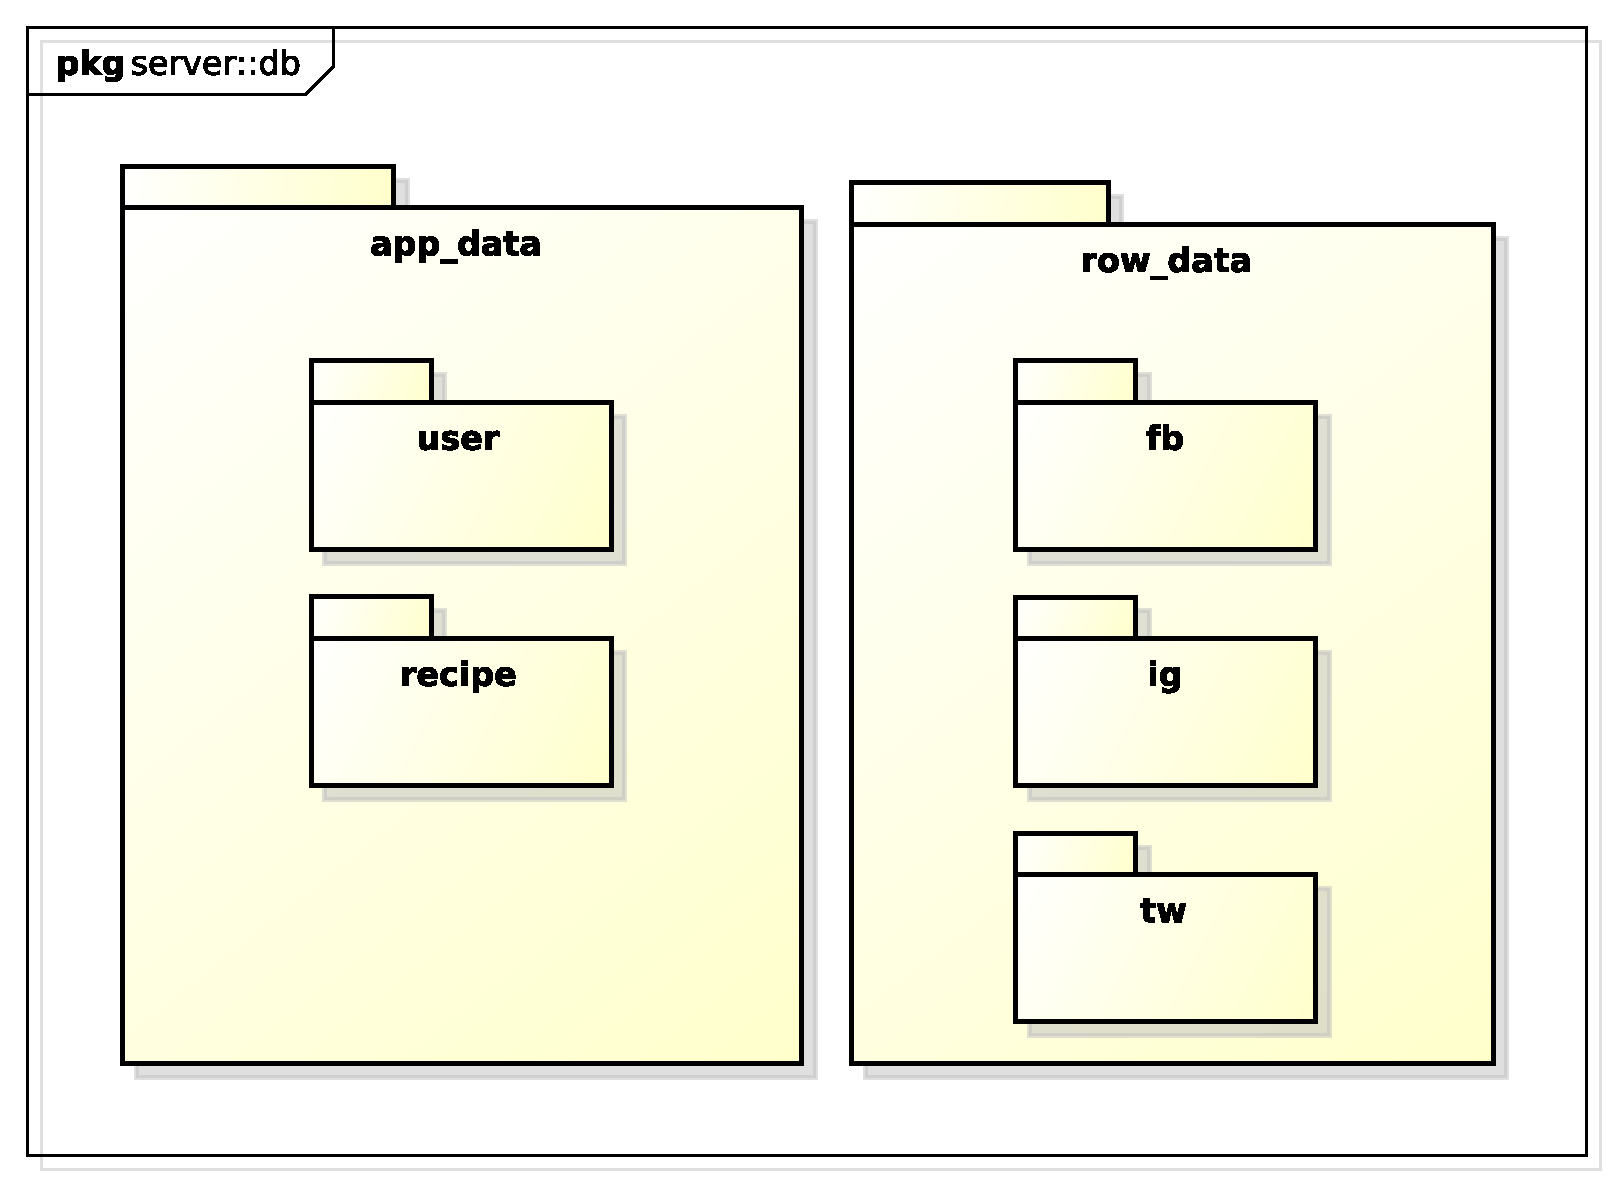
\includegraphics[scale=0.5]{./images/server/db.pdf}}
		\caption{Package - server::db}
	\end{figure}

	\begin{itemize}
		\item \textbf{Descrizione}: è il package che contiene le componenti che gestiscono e mantengono coerente la base di dati. Esse utilizzano standard proprietari Google per la loro implementazione. Sono suddivise in due package uno atto all'immagazzinamento dei dati grezzi, l'altro per la memorizzazione dei parametri del software e degli utenti;
		\item \textbf{Padre}: server;
		\item \textbf{Package contenuti}:
			\begin{itemize}
				\item bdsm\_app::server::app\_data.
				\item bdsm\_app::server::raw\_data;
			\end{itemize}
	\end{itemize}



% subsubsection RAW_DATA
\subsubsection{bdsm\_app::server::db::raw\_data} % (fold)
\label{ssub:bdsm_app_server_raw_model}

	\begin{figure}[htbp]
		\centering
		\centerline{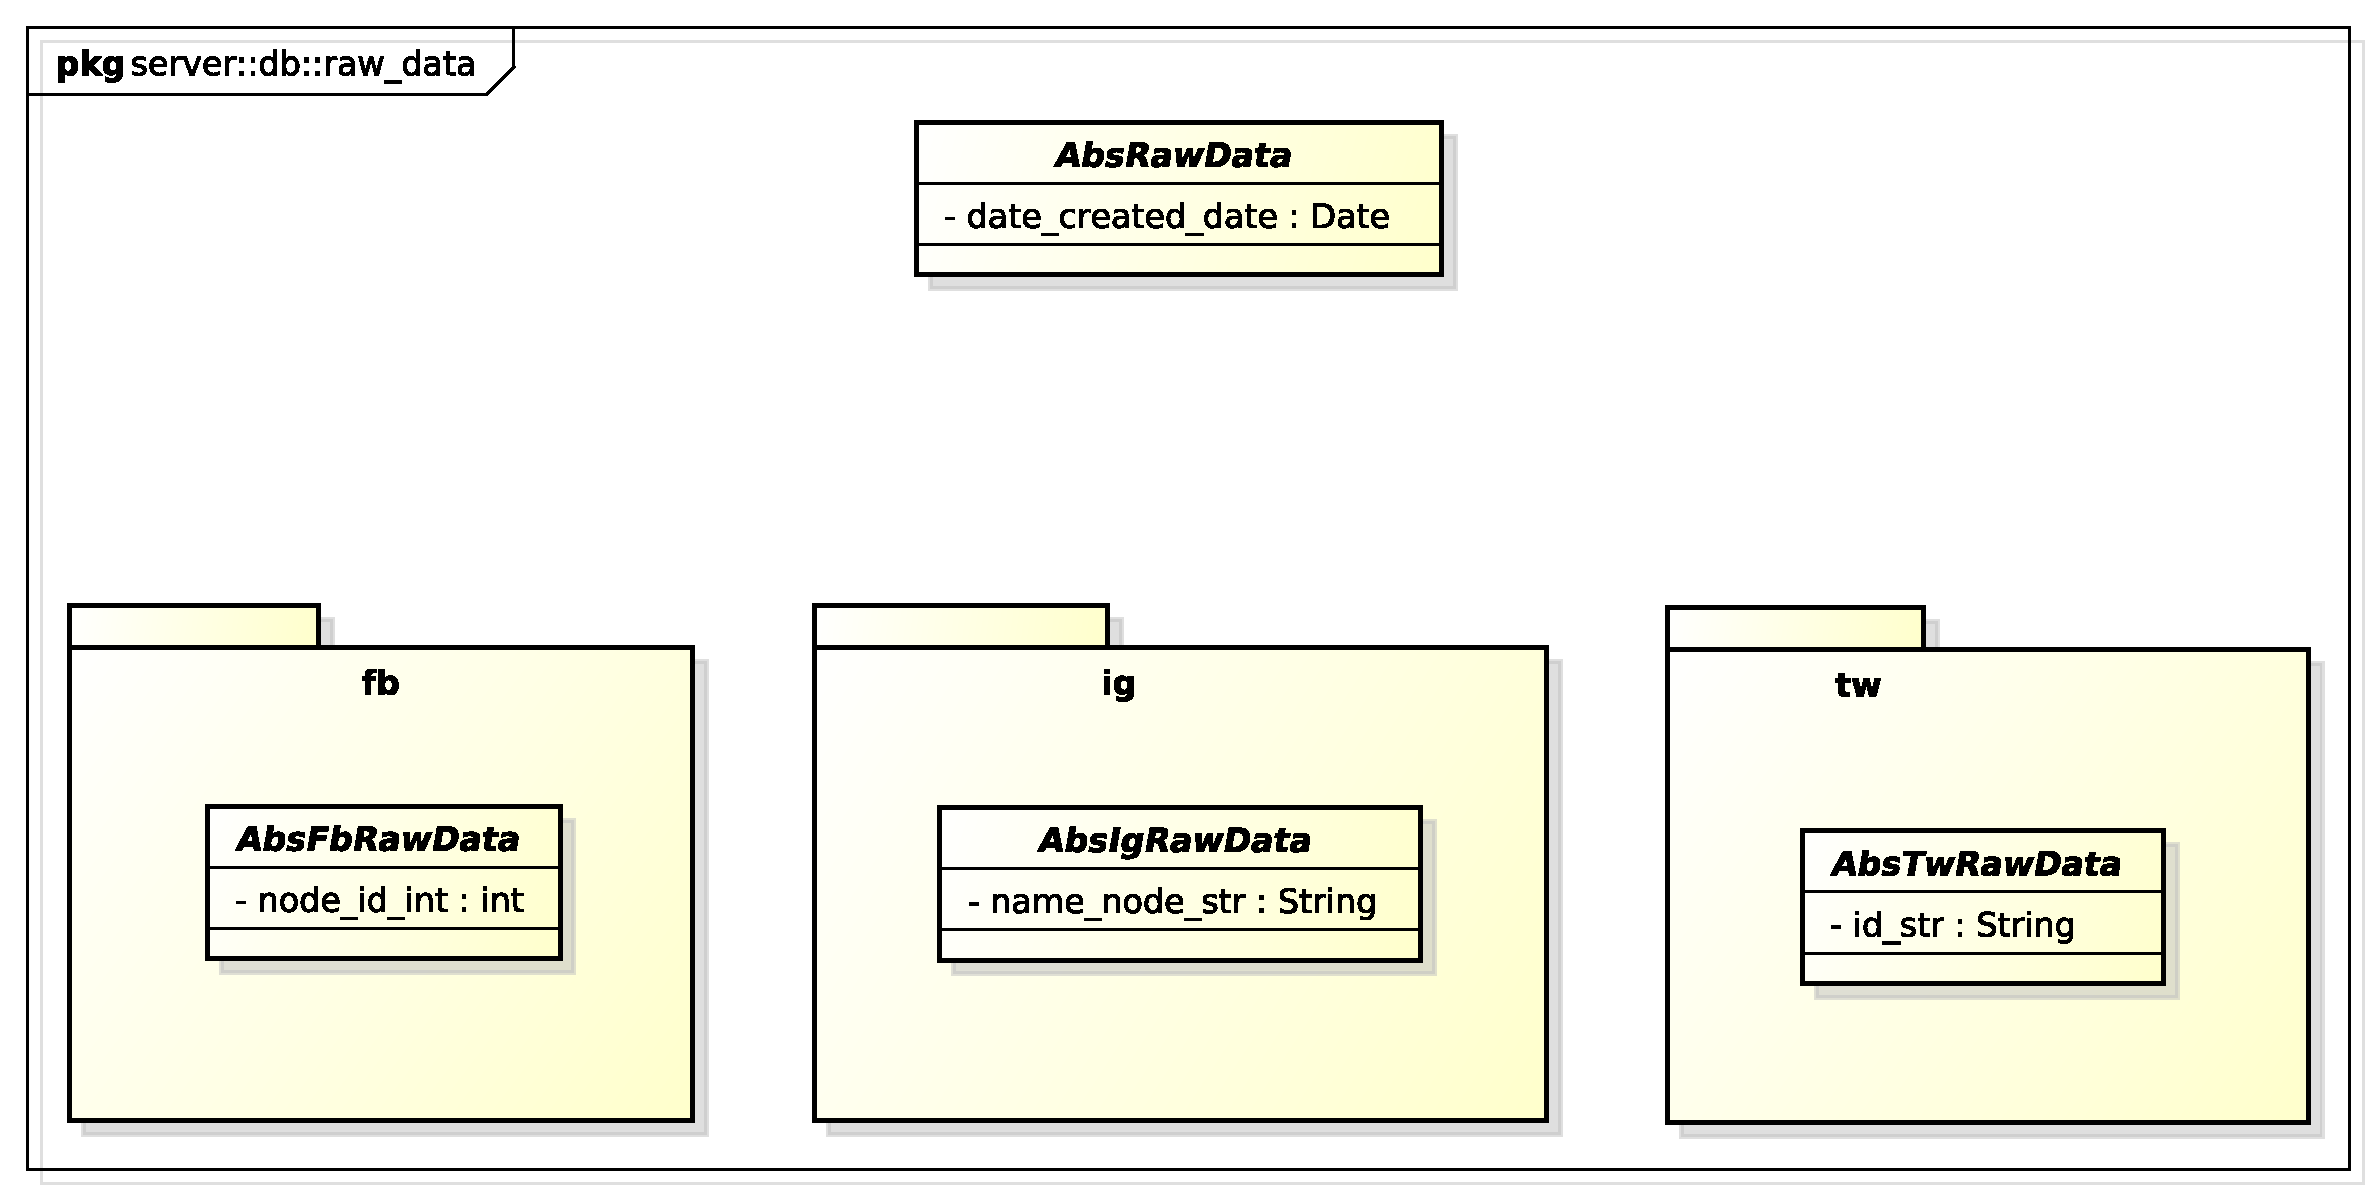
\includegraphics[scale=0.35]{./images/server/raw_data.pdf}}
		\caption{Package - server::db::raw\_data}
	\end{figure}
	\begin{itemize}
	\item \textbf{Descrizione}: Package che definisce il modello dei dati grezzi ricavati dai vari social network;
		\item \textbf{Padre}: server::db;
		\item \textbf{Interazione con altri componenti}: interagisce con il miner il quale salva i dati secondo questo modello, interagisce con l'endpoints il quale interroga la base di dati;
	\end{itemize}


	\paragraph{Classi} % (fold)
		

		\subparagraph{bdsm\_app::server::db::raw\_model::AbsRawData} % (fold)
		\label{subp:bdsm_app_server_raw_model_AbsRawData}
			\begin{itemize}
				\item \textbf{Descrizione}: classe astratta che definisce il modello di un dato grezzo;
				\item \textbf{Utilizzo}: la classe viene istanziata per definire un insieme di dati grezzi. Viene utilizzata come contenitore generico;
				\item \textbf{Relazioni con altre classi}:
					\begin{itemize}
						\item AbsFbRawData;
						\item AbsTwRawData;
						\item AbsIgRawData;
					\end{itemize}
			\end{itemize}


		% subsubsection FACEBOOK


		\begin{figure}[htbp]
			\centering
			\centerline{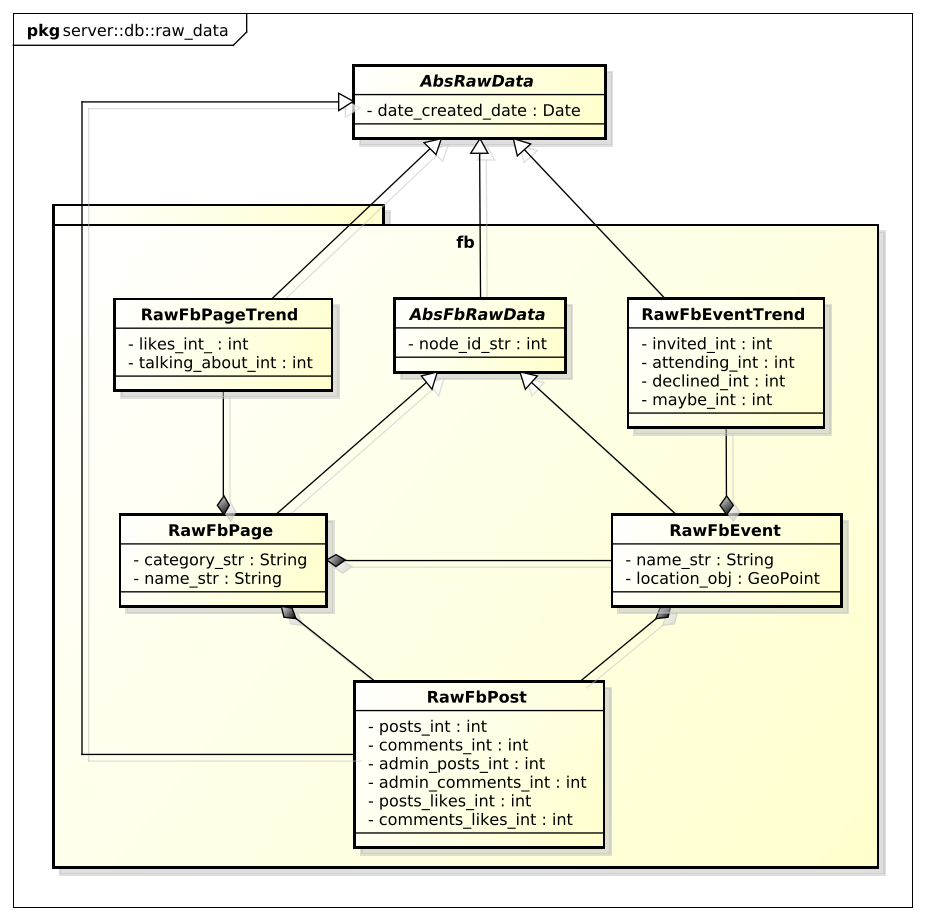
\includegraphics[scale=0.5]{./images/server/raw_data_fb.pdf}}
			\caption{Package - server::db::raw\_data::fb}
		\end{figure}

		
		\subparagraph{server::db::raw\_data::fb::AbsFbRawData} % (fold)
		\label{subp:server_db_raw_data_fb_absfbrawdata}
			\begin{itemize}
				\item \textbf{Descrizione}: classe astratta che definisce il modello dati di Facebook;
				\item \textbf{Utilizzo}: la classe contiene l'id fornito dall'utente il quale permette di identificare univocamente la risorsa nel social media;
				\item \textbf{Classi ereditate}: server::db::raw\_data::AbsRawData
				\item \textbf{Relazioni con altre classi}:
					\begin{itemize}
						\item server::db::raw\_data::fb::RawFbEvent;
						\item server::db::raw\_data::fb::RawFbPage;
					\end{itemize}
			\end{itemize}
		% subparagraph server_db_raw_data_fb_absfbrawdata [end]


		\subparagraph{server::db::raw\_data::fb::RawFbPageTrend} % (fold)
		\label{subp:server_db_raw_data_fb_rowfbpagetrend}
			\begin{itemize}
				\item \textbf{Descrizione}: classe che memorizza i trend di una pagina Facebook;
				\item \textbf{Utilizzo}: la classe viene utilizzata per memorizzare il numero di like e di talking about di ogni singola pagina;
				\item \textbf{Classi ereditate}: server::db::raw\_data::AbsRawData
			\end{itemize}
		% subparagraph server_db_raw_data_fb_rowfbpagetrend [end]


		\subparagraph{server::db::raw\_data::fb::RawFbEventTrend} % (fold)
		\label{subp:server_db_raw_data_fb_rowfbeventtrend}
			\begin{itemize}
				\item \textbf{Descrizione}: classe che memorizza i trend di un evento su Facebook;
				\item \textbf{Utilizzo}: la classe viene utilizzata per memorizzare il numero di utenti invitati, partecipanti e non di un evento;
				\item \textbf{Classi ereditate}: server::db::raw\_data::AbsRawData
			\end{itemize}
		% subparagraph server_db_raw_data_fb_rowfbeventtrend [end]


		\subparagraph{server::db::raw\_data::fb::RawFbPage} % (fold)
		\label{subp:server_db_raw_data_fb_rawfbpage}
			\begin{itemize}
				\item \textbf{Descrizione}: classe delegata alla memorizzazione della pagina Facebook;
				\item \textbf{Utilizzo}: la classe fornisce metodi per memorizzare i dati statici di una pagina Facebook;
				\item \textbf{Classi ereditate}: server::db::raw\_data::AbsFbRawData
				\item \textbf{Relazioni con altre classi}:
					\begin{itemize}
						\item server::db::raw\_data::fb::RawFbEvent;
						\item server::db::raw\_data::fb::RawFbPageTrend;
						\item server::db::raw\_data::fb::RawFbPost;
					\end{itemize}
			\end{itemize}
		% subparagraph server_db_raw_data_fb_rawfbpage [end]


		\subparagraph{server::db::raw\_data::fb::RawFbEvent} % (fold)
		\label{subp:server_db_raw_data_fb_rawfbevent}
			\begin{itemize}
				\item \textbf{Descrizione}: classe delegata alla memorizzazione di un evento Facebook;
				\item \textbf{Utilizzo}: la classe fornisce metodi per memorizzare i dati statici di una pagina evento Facebook;
				\item \textbf{Classi ereditate}: server::db::raw\_data::AbsFbRawData
				\item \textbf{Relazioni con altre classi}:
					\begin{itemize}
						\item server::db::raw\_data::fb::RawFbEventTrend;
						\item server::db::raw\_data::fb::RawFbPost;
					\end{itemize}
			\end{itemize}
		% subparagraph server_db_raw_data_fb_rawfbevent [end]


		\subparagraph{server::db::raw\_data::fb::RawFbPost} % (fold)
		\label{subp:server_db_raw_data_fb_rawfbpost}
			\begin{itemize}
				\item \textbf{Descrizione}: classe delegata alla memorizzazione di un post su Facebook;
				\item \textbf{Utilizzo}: la classe fornisce metodi per sommare i dati statici sui post di Facebook;
			\end{itemize}
		% subparagraph server_db_raw_data_fb_rawfbpost [end]


		% subsubsection INSTAGRAM


		\begin{figure}[htbp]
			\centering
			\centerline{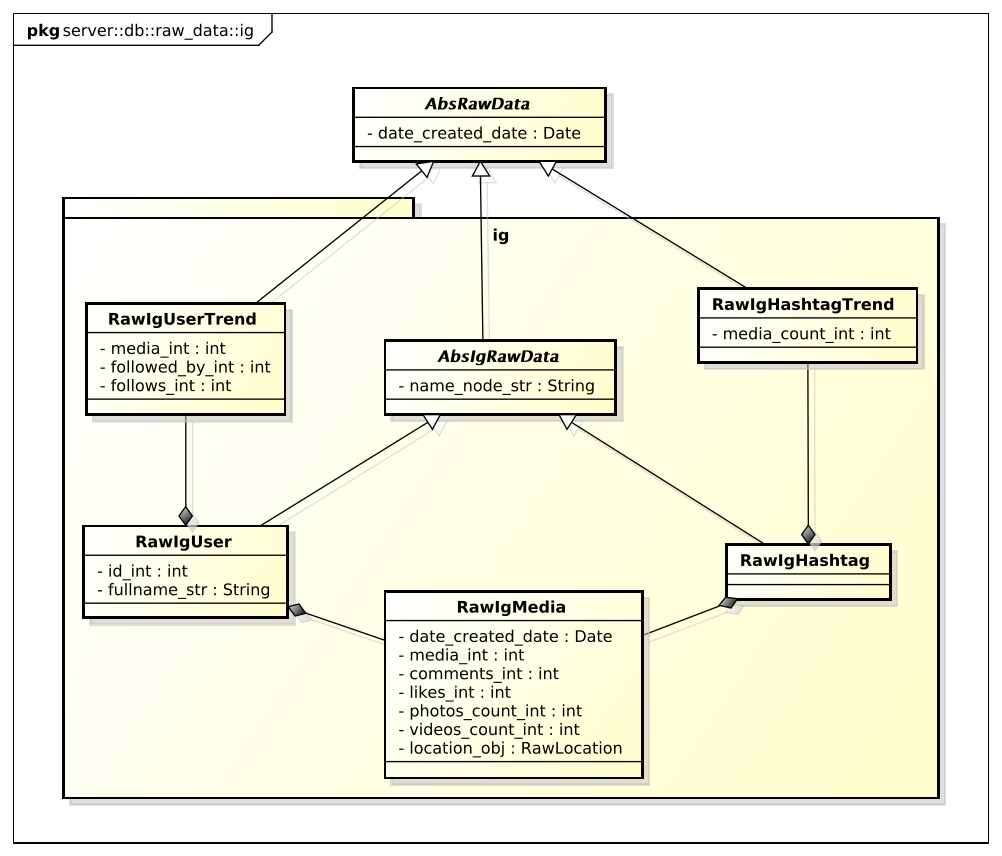
\includegraphics[scale=0.5]{./images/server/raw_data_ig.pdf}}
			\caption{Package - server::db::raw\_data::ig}
		\end{figure}

		
		\subparagraph{server::db::raw\_data::ig::AbsIgRawData} % (fold)
		\label{subp:server_db_raw_data_ig_absigrawdata}
			\begin{itemize}
				\item \textbf{Descrizione}: classe astratta che definisce il modello dati di Instagram;
				\item \textbf{Utilizzo}: la classe contiene l'id fornito dall'utente il quale permette di identificare univocamente la risorsa nel social media;
				\item \textbf{Classi ereditate}: server::db::raw\_data::AbsRawData
				\item \textbf{Relazioni con altre classi}:
					\begin{itemize}
						\item server::db::raw\_data::ig::RawIgUser;
						\item server::db::raw\_data::ig::RawIgHashtag;
					\end{itemize}
			\end{itemize}
		% subparagraph server_db_raw_data_ig_absigrawdata [end]


		\subparagraph{server::db::raw\_data::ig::RawIgUserTrend} % (fold)
		\label{subp:server_db_raw_data_ig_rawigusertrend}
			\begin{itemize}
				\item \textbf{Descrizione}: classe che memorizza i trend di un utente Instagram;
				\item \textbf{Utilizzo}: la classe viene utilizzata per memorizzare il numero di media, di followed e follows di una determinata persona;
				\item \textbf{Classi ereditate}: server::db::raw\_data::AbsRawData
			\end{itemize}
		% subparagraph server_db_raw_data_ig_rawigusertrend [end]


		\subparagraph{server::db::raw\_data::ig::RawIgHashtagTrend} % (fold)
		\label{subp:server_db_raw_data_ig_rawighashtagtrend}
			\begin{itemize}
				\item \textbf{Descrizione}: classe che memorizza i trend di un hastag Instagram;
				\item \textbf{Utilizzo}: la classe viene utilizzata per memorizzare il numero di media caricati di un determinato hashtag;
				\item \textbf{Classi ereditate}: server::db::raw\_data::AbsRawData
			\end{itemize}
		% subparagraph server_db_raw_data_ig_rawighashtagtrend [end]



		\subparagraph{server::db::raw\_data::ig::RawIgUser} % (fold)
		\label{subp:server_db_raw_data_ig_rawiguser}
			\begin{itemize}
				\item \textbf{Descrizione}: classe che definisce le proprietà di un utente Instagram;
				\item \textbf{Utilizzo}: la classe viene utilizzata per fornire una descrizione minimale dell'utente Instagram;
				\item \textbf{Classi ereditate}: server::db::raw\_data::AbsIgRawData
				\item \textbf{Relazioni con altre classi}:
					\begin{itemize}
						\item server::db::raw\_data::ig::RawIgUserTrend;
						\item server::db::raw\_data::ig::RawIgMedia;
					\end{itemize}
			\end{itemize}
		% subparagraph server_db_raw_data_ig_rawiguser [end]


		\subparagraph{server::db::raw\_data::ig::RawIgHashtag} % (fold)
		\label{subp:server_db_raw_data_ig_rawighashtag}
			\begin{itemize}
				\item \textbf{Descrizione}: classe che definisce le proprietà di un hashtag su Instagram;
				\item \textbf{Utilizzo}: la classe viene utilizzata per fornire una descrizione minimale dell'hashtag su Instagram;
				\item \textbf{Classi ereditate}: server::db::raw\_data::AbsIgRawData
				\item \textbf{Relazioni con altre classi}:
					\begin{itemize}
						\item server::db::raw\_data::ig::RawIgHashtagTrend;
						\item server::db::raw\_data::ig::RawIgMedia;
					\end{itemize}
			\end{itemize}
		% subparagraph server_db_raw_data_ig_rawighashtag [end]


		\subparagraph{server::db::raw\_data::ig::RawIgMedia} % (fold)
		\label{subp:server_db_raw_data_ig_rawigmedia}
			\begin{itemize}
				\item \textbf{Descrizione}: classe che definisce le proprietà di un media su Instagram;
				\item \textbf{Utilizzo}: la classe viene utilizzata per fornire una descrizione dettagliata di un media caricato da un utente specifico su Instagram. Vengono forniti metodi automatici per il conteggio dei parametri che verranno utilizzati per seguire un trend;
			\end{itemize}
		% subparagraph server_db_raw_data_ig_rawigmedia [end]


		% subsubsection TWITTER


		\begin{figure}[htbp]
			\centering
			\centerline{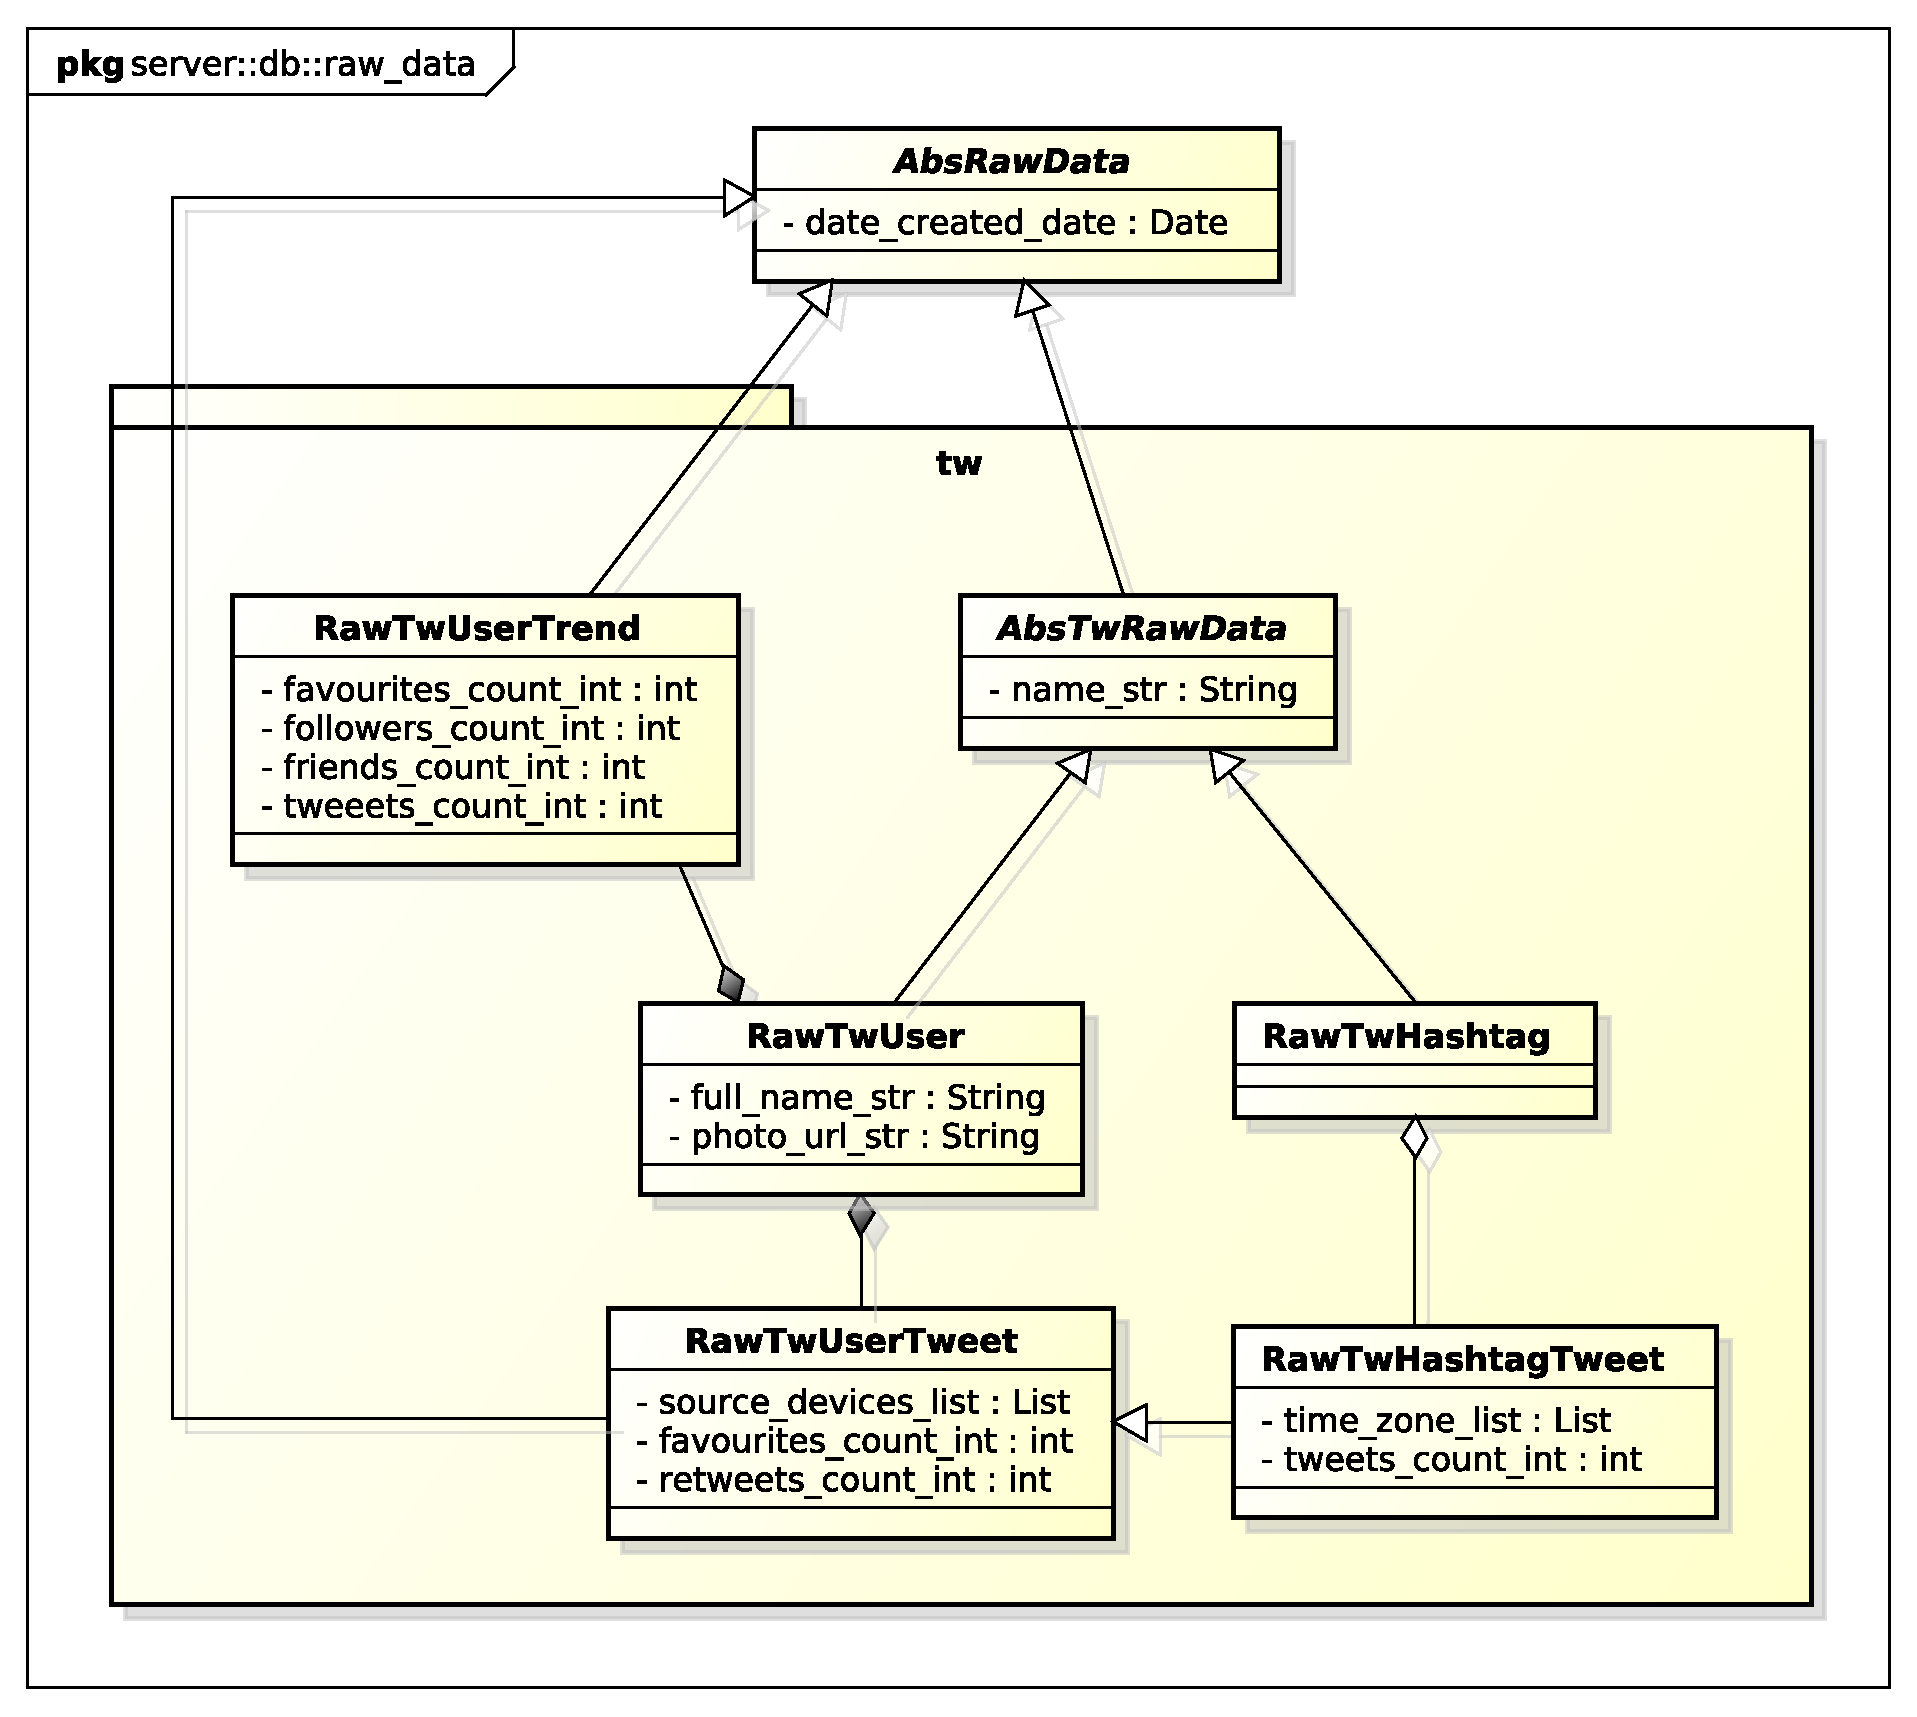
\includegraphics[scale=0.45]{./images/server/raw_data_tw.pdf}}
			\caption{Package - server::db::raw\_data::tw}
		\end{figure}

		
		\subparagraph{server::db::raw\_data::tw::AbsTwRawData} % (fold)
		\label{subp:server_db_raw_data_tw_abstwrawdata}
			\begin{itemize}
				\item \textbf{Descrizione}: classe astratta che definisce il modello dati di Twitter;
				\item \textbf{Utilizzo}: la classe contiene l'id fornito dall'utente il quale permette di identificare univocamente la risorsa nel social media;
				\item \textbf{Classi ereditate}: server::db::raw\_data::AbsRawData
				\item \textbf{Relazioni con altre classi}:
					\begin{itemize}
						\item server::db::raw\_data::tw::RawTwUser;
						\item server::db::raw\_data::tw::RawTwHashtag;
					\end{itemize}
			\end{itemize}
		% subparagraph server_db_raw_data_tw_abstwrawdata [end]


		\subparagraph{server::db::raw\_data::tw::RawTwUserTrend} % (fold)
		\label{subp:server_db_raw_data_tw_rawigusertrend}
			\begin{itemize}
				\item \textbf{Descrizione}: classe che memorizza i trend di un utente Twitter;
				\item \textbf{Utilizzo}: la classe viene utilizzata per memorizzare il numero di favoriti, di followers, di friends e statuses di una determinata persona;
				\item \textbf{Classi ereditate}: server::db::raw\_data::AbsRawData
			\end{itemize}
		% subparagraph server_db_raw_data_tw_rawigusertrend [end]


		\subparagraph{server::db::raw\_data::tw::RawTwHashtagTrend} % (fold)
		\label{subp:server_db_raw_data_tw_rawighashtagtrend}
			\begin{itemize}
				\item \textbf{Descrizione}: classe che memorizza i trend di un hashtag su Twitter;
				\item \textbf{Utilizzo}: la classe viene utilizzata per memorizzare il numero di favoriti, di followers e statuses di un determinato hashtag;
				\item \textbf{Classi ereditate}: server::db::raw\_data::AbsRawData
			\end{itemize}
		% subparagraph server_db_raw_data_tw_rawighashtagtrend [end]


		\subparagraph{server::db::raw\_data::tw::RawTwUser} % (fold)
		\label{subp:server_db_raw_data_tw_rawtwuser}
			\begin{itemize}
				\item \textbf{Descrizione}: classe che definisce le proprietà di un utente Twitter;
				\item \textbf{Utilizzo}: la classe viene utilizzata per fornire una descrizione completa dell'utente Twitter. Vengono forniti metodi automatici per il conteggio dei parametri che verranno utilizzati per seguire un trend;;
				\item \textbf{Classi ereditate}: server::db::raw\_data::AbsTwRawData
				\item \textbf{Relazioni con altre classi}:
					\begin{itemize}
						\item server::db::raw\_data::tw::RawTwUserTrend;
						\item server::db::raw\_data::tw::RawTwUserTweet;
					\end{itemize}
			\end{itemize}
		% subparagraph server_db_raw_data_tw_rawtwuser [end]


		\subparagraph{server::db::raw\_data::tw::RawTwHashtag} % (fold)
		\label{subp:server_db_raw_data_tw_rawtwhashtag}
			\begin{itemize}
				\item \textbf{Descrizione}: classe che definisce le proprietà di un hashtag su Twitter;
				\item \textbf{Utilizzo}: la classe viene utilizzata per fornire una descrizione minimale di un hashtag su Twitter. Vengono forniti metodi automatici per il conteggio dei parametri che verranno utilizzati per seguire un trend;;
				\item \textbf{Classi ereditate}: server::db::raw\_data::AbsTwRawData
				\item \textbf{Relazioni con altre classi}:
					\begin{itemize}
						\item server::db::raw\_data::tw::RawTwHashtagTrend;
						\item server::db::raw\_data::tw::RawTwHashtagTweet;
					\end{itemize}
			\end{itemize}
		% subparagraph server_db_raw_data_tw_rawtwhashtag [end]


		\subparagraph{server::db::raw\_data::tw::RawTwUserTweet} % (fold)
		\label{subp:server_db_raw_data_tw_rawtwusertweet}
			\begin{itemize}
				\item \textbf{Descrizione}: classe che definisce le proprietà di un insieme di tweet su Twitter;
				\item \textbf{Utilizzo}: la classe viene utilizzata per fornire una descrizione dettagliata di un tweet creato da un utente specifico su Twitter;
			\end{itemize}
		% subparagraph server_db_raw_data_tw_rawtwusertweet [end]


		\subparagraph{server::db::raw\_data::tw::RawTwHashtagTweet} % (fold)
		\label{subp:server_db_raw_data_tw_rawtwhashtagtweet}
			\begin{itemize}
				\item \textbf{Descrizione}: classe che definisce le proprietà di un insieme di hashtag su Twitter;
				\item \textbf{Utilizzo}: la classe viene utilizzata per fornire una descrizione della locazione spaziale di un tweet relativo all'hashtag su Twitter;
				\item \textbf{Classi ereditate}: server::db::raw\_data::RawTwUserTweet
			\end{itemize}
		% subparagraph server_db_raw_data_tw_rawtwhashtagtweet [end]











\subsubsection{bdsm\_app::server::db::app\_data} % (fold)
\label{ssub:bdsm_app_server_app_data}


	\begin{figure}[htbp]
		\centering
		\centerline{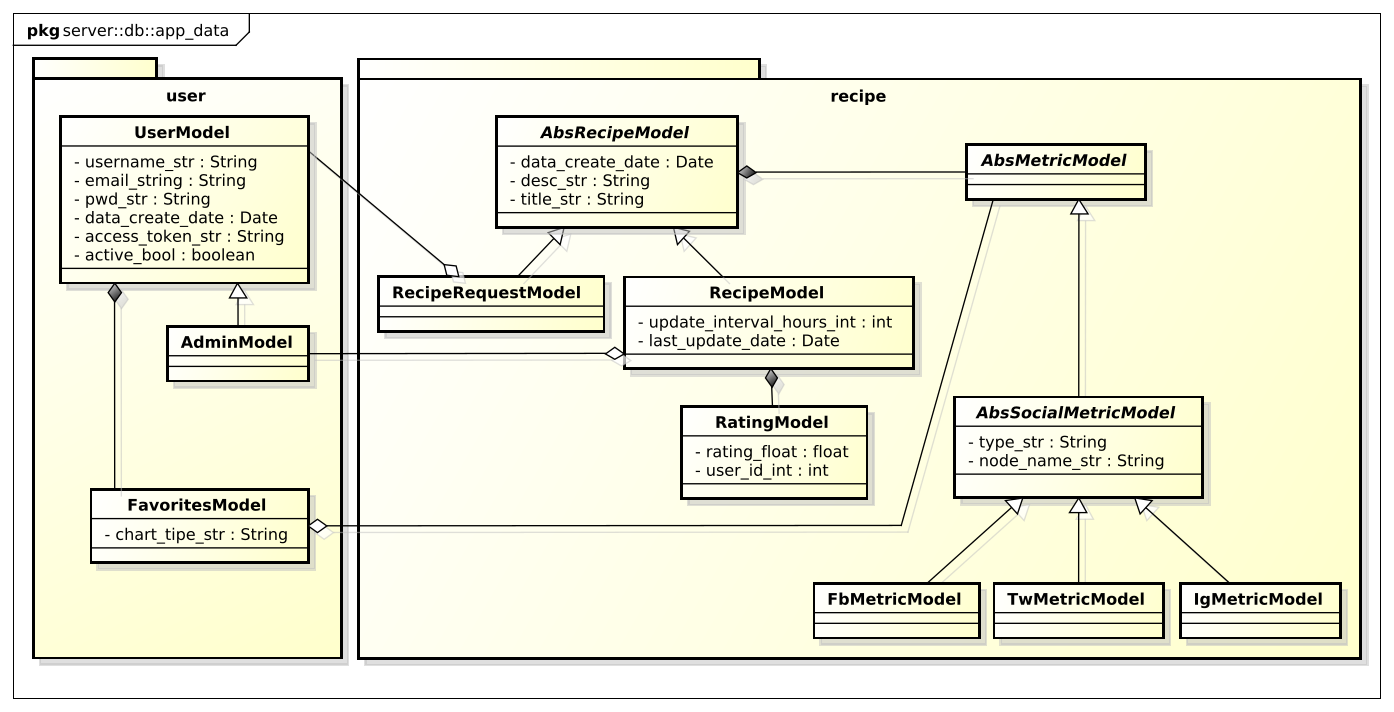
\includegraphics[scale=0.38]{./images/server/app_data.pdf}}
		\caption{Package - server::db::app\_data}
	\end{figure}


	\begin{itemize}
		\item \textbf{Descrizione}: è il package che contiene le informazioni di tutti gli utenti registrati e le loro preferenze. Contiene inoltre il modello di recipe che l'amministratore decide di creare;
		\item \textbf{Padre}: server;
		\item \textbf{Package contenuti}
			\begin{itemize}
				\item user;
				\item recipe;
			\end{itemize}
		\item \textbf{Interazione con altri componenti}: interagisce con tutti i componenti del server in quanto fornisce i metodi per manipolare tutti i dati da memorizzare;
	\end{itemize}
	% subsubsection bdsm_app_server_app_data [end]


	\paragraph{Classi} % (fold)

		\subparagraph{server::db::app\_data::user::UserModel} % (fold)
		\label{subp:server_db_app_data_user_user_model}
			\begin{itemize}
				\item \textbf{Descrizione}: classe che fornisce i metodi per memorizzare gli utenti all'interno della base di dati;
				\item \textbf{Utilizzo}: la classe conterrà i metodi per la creazione, eliminazione, modifica degli account utente;
				\item \textbf{Relazioni con altre classi}:
					\begin{itemize}
						\item server::db::app\_data::user::Favorites;
						\item server::db:::app\data::user::AdminModel;
						\item server::db::app\data::recipe::RecipeRequestModel;
					\end{itemize}
			\end{itemize}
		% subparagraph server_db_app_data_user_user_model [end]


		\subparagraph{server::db::app\_data::user::AdminModel} % (fold)
		\label{subp:server_db_app_data_user_admin_model}
			\begin{itemize}
				\item \textbf{Descrizione}: classe che fornisce i metodi per memorizzare gli utenti amministratori all'interno della base di dati;
				\item \textbf{Utilizzo}: la classe specializza l'utente amministratore. Viene implementata con dei metodi per l'aggiunta la modifica e la rimozione;
				\item \textbf{Classi ereditate}: server::db::app\_data::user::UserModel;
				\item \textbf{Relazioni con altre classi}:
					\begin{itemize}
						\item server::db::app\_data::recipe::RecipeModel;
					\end{itemize}
			\end{itemize}
		% subparagraph server_db_app_data_user_admin_model [end]


		\subparagraph{server::db::app\_data::user::Favorites} % (fold)
		\label{subp:server_db_app_data_user_favorites}
			\begin{itemize}
				\item \textbf{Descrizione}: classe che memorizzare i preferiti dell'utente;
				\item \textbf{Utilizzo}: la classe  permette all'utente di aggiungere dei modelli di view nei preferiti. Contiene metodi per l'inserimento e rimozione di preferiti;
				\item \textbf{Relazioni con altre classi}:
					\begin{itemize}
						\item server::db::app\_data::recipe::AbsMetricModel;
					\end{itemize}
			\end{itemize}
		% subparagraph server_db_app_data_user_favorites [end]


		\subparagraph{server::db::app\_data::recipe::AbsRecipeModel} % (fold)
		\label{subp:server_db_app_data_recipe_absrecipemodel}
			\begin{itemize}
				\item \textbf{Descrizione}: classe astratta che rappresenta il padre ;
				\item \textbf{Utilizzo}: la classe specializza la ricetta identificando l'utente amministratore che l'ha creata ed i campi dati necessari per tenere memorizzato nella base di dati le operazioni da effettuare successivamente;
				\item \textbf{Relazioni con altre classi}:
					\begin{itemize}
						\item server::db::app\_data::recipe::RecipeModel;
						\item server::db::app\_data::recipe::RecipeRequestModel;
						\item server::db::app\_data::recipe::AbsMetricModel;
					\end{itemize}
			\end{itemize}
		% subparagraph server_db_app_data_recipe_absrecipemodel [end]


		\subparagraph{server::db::app\_data::recipe::RecipeRequestModel} % (fold)
		\label{subp:server_db_app_data_recipe_reciperequestmodel}
			\begin{itemize}
				\item \textbf{Descrizione}: classe che rappresenta la richiesta da parte dell'utente di creazione di una nuova ricetta;
				\item \textbf{Utilizzo}: la classe specializza la richiesta identificandone l'utente;
				\item \textbf{Classi ereditate}: server::db::app\_data::recipe::AbsRecipeModel;
			\end{itemize}
		% subparagraph server_db_app_data_recipe_reciperequestmodel [end]


		\subparagraph{server::db::app\_data::recipe::RecipeModel} % (fold)
		\label{subp:server_db_app_data_recipe_recipemodel}
			\begin{itemize}
				\item \textbf{Descrizione}: classe che rappresenta il modello di ricetta;
				\item \textbf{Utilizzo}: la classe specializza la ricetta. Vengono forniti i campi dati per il possibile incremento temporale dei dati;
				\item \textbf{Classi ereditate}: server::db::app\_data::recipe::AbsRecipeModel;
			\end{itemize}
		% subparagraph server_db_app_data_recipe_recipemodel [end]


		\subparagraph{server::db::app\_data::recipe::AbsMetricModel} % (fold)
		\label{subp:server_db_app_data_recipe_absmetricmodel}
			\begin{itemize}
				\item \textbf{Descrizione}: classe astratta che rappresenta il modello di metrica da applicare alla ricetta;
				\item \textbf{Utilizzo}: la classe ha il compito di inglobare tutte le sotto-metriche e non solo quelle derivate dai social media;
				\item \textbf{Relazioni con altre classi}:
					\begin{itemize}
						\item server::db::app\_data::recipe::AbsSocialMetricModel;
					\end{itemize}
			\end{itemize}
		% subparagraph server_db_app_data_recipe_absmetricmodel [end]


		\subparagraph{server::db::app\_data::recipe::AbsSocialMetricModel} % (fold)
		\label{subp:server_db_app_data_recipe_abssocialmetricmodel}
			\begin{itemize}
				\item \textbf{Descrizione}: classe astratta identifica le metriche dei social media;
				\item \textbf{Utilizzo}: la classe ha il compito di raggruppare i social media da rappresentare e identificarli univocamente;
				\item \textbf{Classi ereditate}: server::db::app\_data::recipe::AbsMetricModel;
				\item \textbf{Relazioni con altre classi}:
					\begin{itemize}
						\item server::db::app\_data::recipe::FbMetricModel;
						\item server::db::app\_data::recipe::IgMetricModel;
						\item server::db::app\_data::recipe::TwMetricModel;
					\end{itemize}
			\end{itemize}
		% subparagraph server_db_app_data_recipe_abssocialmetricmodel [end]


		\subparagraph{server::db::app\_data::recipe::FbMetricModel} % (fold)
		\label{subp:server_db_app_data_recipe_fbmetricmodel}
			\begin{itemize}
				\item \textbf{Descrizione}: classe che identifica le metriche dei social Facebook;
				\item \textbf{Utilizzo}: la classe ha il compito di identificare univocamente l'id della pagina o l'id dell'evento da analizzare. La classe fornisce metodi per l'aggiunta e la rimozione ricorsiva in caso di cancellazione;
				\item \textbf{Classi ereditate}: server::db::app\_data::recipe::AbsSocialMetricModel;
			\end{itemize}
		% subparagraph server_db_app_data_recipe_fbmetricmodel [end]


		\subparagraph{server::db::app\_data::recipe::IgMetricModel} % (fold)
		\label{subp:server_db_app_data_recipe_igmetricmodel}
			\begin{itemize}
				\item \textbf{Descrizione}: classe che identifica le metriche dei social Instagram;
				\item \textbf{Utilizzo}: la classe ha il compito di identificare univocamente l'id della pagina o l'hashtag da analizzare. La classe fornisce metodi per l'aggiunta e la rimozione ricorsiva in caso di cancellazione;
				\item \textbf{Classi ereditate}: server::db::app\_data::recipe::AbsSocialMetricModel;
			\end{itemize}
		% subparagraph server_db_app_data_recipe_igmetricmodel [end]


		\subparagraph{server::db::app\_data::recipe::TwMetricModel} % (fold)
		\label{subp:server_db_app_data_recipe_twmetricmodel}
			\begin{itemize}
				\item \textbf{Descrizione}: classe che identifica le metriche dei social Twitter;
				\item \textbf{Utilizzo}: la classe ha il compito di identificare univocamente l'id della pagina o l'hashtag da analizzare. La classe fornisce metodi per l'aggiunta e la rimozione ricorsiva in caso di cancellazione;
				\item \textbf{Classi ereditate}: server::db::app\_data::recipe::AbsSocialMetricModel;
			\end{itemize}
		% subparagraph server_db_app_data_recipe_twmetricmodel [end]